%%%%%%%%%%%%  METHODS  %%%%%%%%%%%% 




%----------------------------------------------------------------------------------------
\subsection{Sediments trap data}

Sediments traps consist of an upward-facing funnel that directs sinking organic and inorganic particulate material towards a sampling bottle. 
Traps are moored at a specific depth in the water column (usually below the euphotic zone or mixed layer) and anchored to a particular location. %REF
Each trap usually contains several collecting bottles to record the changes in sinking flux with time, typically at the resolution of weeks. %REF
Therefore, sediment traps provide continuous time series of settling foraminiferal shell fluxes (expressed as number of shells per $m^2$ per day). 

Shell fluxes represent the settling of dead foraminifera and are strictly speaking not directly a measure of abundance of foraminifera in the water column \cite{jonkers2015global}. However, given the short life span of foraminifera (typically one month \citep{hemleben1989modern}), the fluxes are likely to be a good proxy for populational abundance. Moreover, to be able to compare fluxes of different species, we assume that species have similar life spans. This means that similar fluxes (i.e. species dying synchronously) indicate that species grow and reach different life stages (juvenile, adults) also synchronously.

%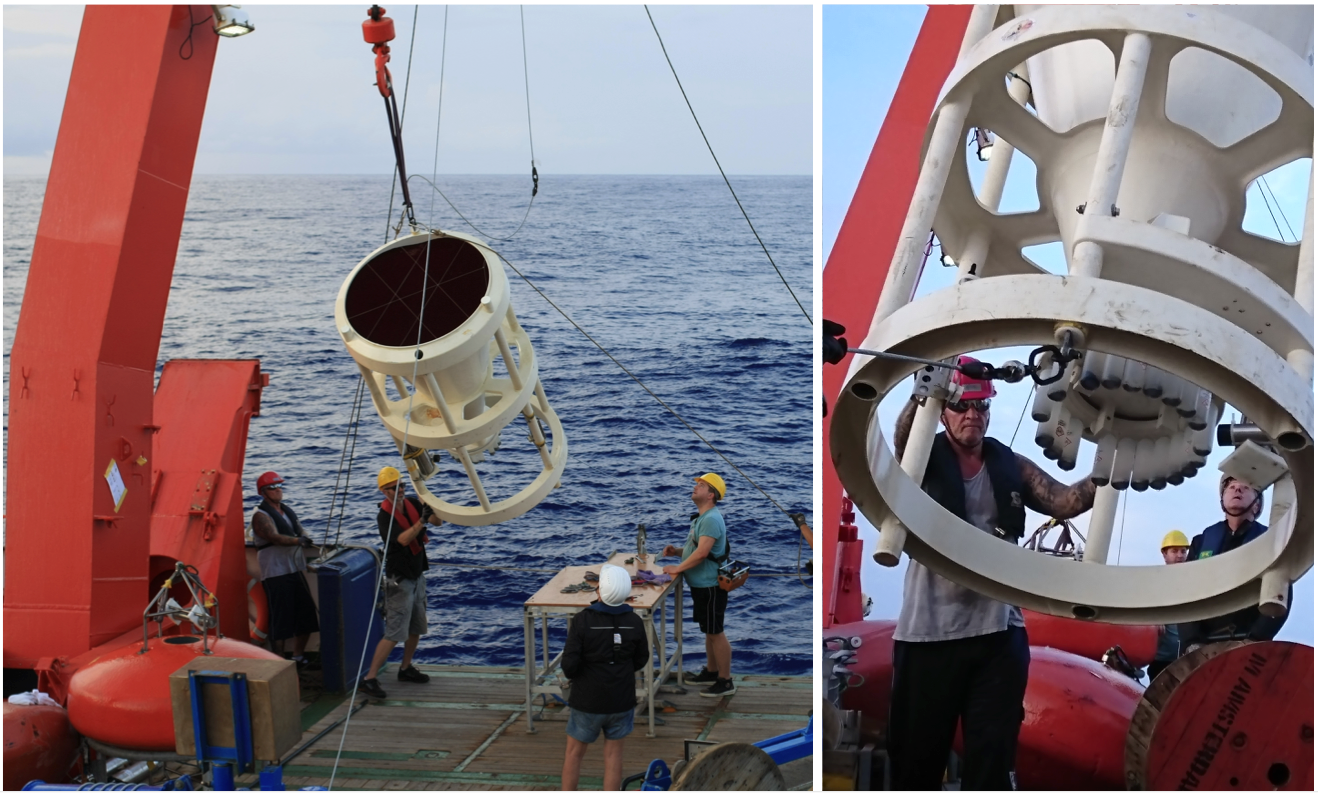
\includegraphics[width=1\textwidth]{sed_trap.png}
%\caption{\label{fig:trap} Recovery of sediment trap during the German Research Cruise M140 in the North Atlantic, crew in the \textit{RV} Meteor, August 2017. \textbf{Left}: sediment trap has a sampling area of $1 m^2$, \textbf{Right}: 20 bottles with samples, note the four missing bottles.}

We used the data of 35 globally distributed moored sediment trap time series (Fig. \ref{fig:map}, compiled by \citealt{jonkers2015global}). All the traps have duration of at least one year; and traps 36 and 37 were excluded from this study because they contain only one polar species. Further information about each trap (\textit{e.g.} location, resolution, total period of sampling) can be found in Table \ref{table:traps_data}. Figure \ref{fig:NB67_series} shows an example of the data gathered by trap no.1 in the North Atlantic. 
% Jonkers 2015: Traps close to the sea floor or in the vicinity of (steep) topography that showed the influence of resuspended material (for instance, the presence of benthic Foraminifera) were not considered. In cases were multiple sediment traps were deployed at different depths on the same mooring, we report data from the shallowest trap as this (likely) reduces the catchment area of the trap and the data hence reflect local conditions more closely.

\begin{figure}
\centering
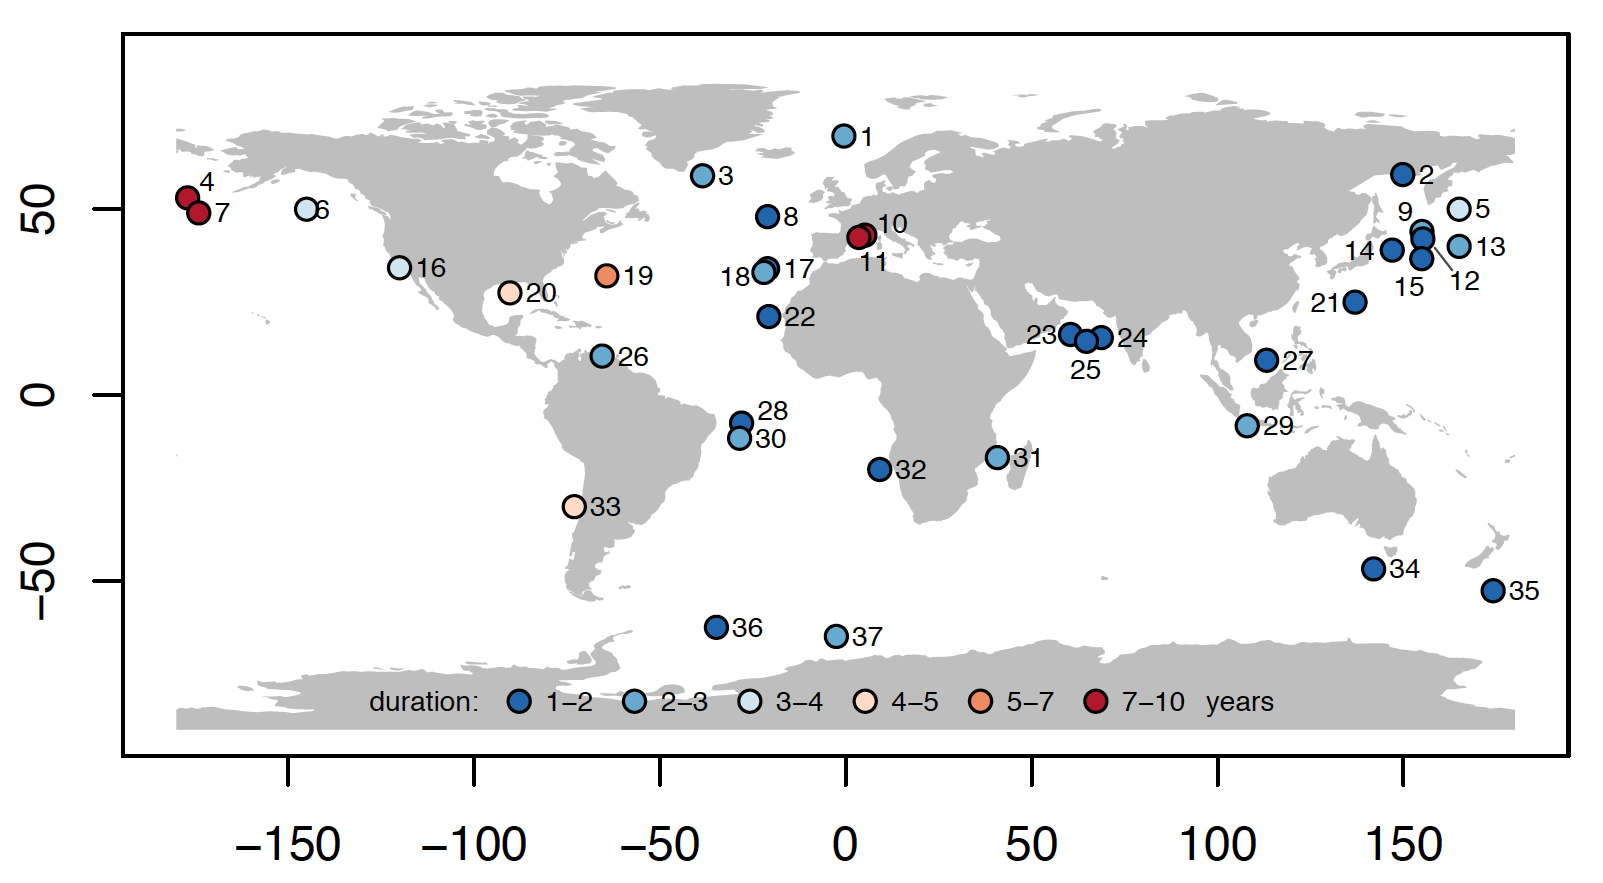
\includegraphics[width=1\textwidth]{traps_map.png}
\caption{\label{fig:map} Distribution and total duration of sediment trap time series used in this study. Figure taken from \citep{jonkers2015global}. Traps 36 and 37 were excluded from this study because they contain only one species. \textcolor{red}{(plot this map myself)}}
\end{figure}

\begin{table}
\footnotesize
\caption{\label{table:traps_data} Meta-data of sediment traps taken from \citep{jonkers2015global}. Columns: \textbf{Trap number} as in Figure \ref{fig:map}; \textbf{Trap name}; Coordinates (\textbf{Lat, Lon}); \textbf{resolution}: mean period (in days) that each sample (bottle) in the trap was open; \textbf{length days}: total period trap was open (in days); \textbf{length years}: total period in years; \textbf{length series}: total number of samples collected in each trap (length of the time-series); \textbf{from, to}: year interval when trap was active; \textbf{all ssp}: whether all species were identified in each trap, "NO" means that just dominant species were picked.}
\makebox[\linewidth]{ % put table in middle of the page
\begin{tabular}{rlllrrrrrrl}
  \hline
Trap & Trap & Lat & Lon & resolution & length & length & length & from & to & all ssp \\ 
no.  & name &  &  & days & days & years & series &  &   &  \\ 
  \hline
  1 & NB67 & 69.69 & -0.47 & 18.20 & 787 & 2.20 &  32 & 1991 & 1993 & YES \\ 
    2 & OKH & 59.32 & 149.83 & 16.40 & 365 & 1.00 &  21 & 1990 & 1991 & YES \\ 
    3 & IRM & 59.00 & -38.50 & 16.00 & 1372 & 3.80 &  58 & 2003 & 2007 & NO \\ 
    4 & AB & 53.05 & -177.00 & 26.90 & 3264 & 8.90 & 105 & 1990 & 1999 & NO \\ 
    5 & PAC50 & 50.00 & 165.00 & 15.50 & 1287 & 3.50 &  69 & 1997 & 2001 & NO \\ 
    6 & PAPA & 50.00 & -145.00 & 12.80 & 1437 & 3.90 &  82 & 1982 & 1986 & NO \\ 
    7 & SA & 49.00 & -174.00 & 26.80 & 3267 & 9.00 & 101 & 1990 & 1999 & NO \\ 
    8 & JGOFS48 & 48.00 & -21.00 & 12.80 & 377 & 1.00 &  26 & 1989 & 1990 & YES \\ 
    9 & PACKNOT & 44.00 & 155.00 & 15.40 & 893 & 2.40 &  52 & 1997 & 2000 & NO \\ 
   10 & LIP & 43.02 & 5.18 & 27.80 & 4457 & 12.20 & 116 & 1993 & 2006 & YES \\ 
   11 & LIL & 42.41 & 3.54 & 22.50 & 4167 & 11.40 & 151 & 1993 & 2005 & YES \\ 
   12 & WCT6 & 42.01 & 155.24 & 19.10 & 381 & 1.00 &  19 & 1999 & 2000 & YES \\ 
   13 & PAC40 & 40.00 & 165.00 & 16.50 & 952 & 2.60 &  44 & 1997 & 2000 & NO \\ 
   14 & WCT2 & 39.00 & 147.00 & 14.20 & 628 & 1.70 &  40 & 1997 & 1999 & PROB \\ 
   15 & WCT7 & 36.69 & 154.94 & 18.80 & 375 & 1.00 &  19 & 1999 & 2000 & PROB \\ 
   16 & SBB & 34.25 & -120.00 & 10.90 & 2144 & 5.90 &  93 & 1993 & 1999 & NO \\ 
   17 & JGOFS34 & 34.00 & -21.00 & 12.80 & 377 & 1.00 &  26 & 1989 & 1990 & YES \\ 
   18 & L1 & 33.00 & -22.00 & 21.80 & 767 & 2.10 &  35 & 2002 & 2004 & YES \\ 
   19 & BATS & 32.08 & -64.25 & 58.60 & 2232 & 6.10 &  31 & 1978 & 1984 & PROB \\ 
   20 & GOM & 27.50 & -90.30 & 7.30 & 2245 & 6.20 & 238 & 2008 & 2014 & NO \\ 
   21 & WCT1 & 25.00 & 137.00 & 14.10 & 612 & 1.70 &  37 & 1997 & 1999 & PROB \\ 
   22 & CB & 21.13 & -20.67 & 17.90 & 753 & 2.10 &  38 & 1989 & 1991 & NO \\ 
   23 & WAST & 16.32 & 60.47 & 13.30 & 529 & 1.40 &  38 & 1986 & 1987 & YES \\ 
   24 & EAST & 15.47 & 68.75 & 11.70 & 527 & 1.40 &  38 & 1986 & 1987 & YES \\ 
   25 & CAST & 14.47 & 64.75 & 12.20 & 516 & 1.40 &  32 & 1986 & 1987 & YES \\ 
   26 & CAR & 10.50 & -65.50 & 12.40 & 1089 & 3.00 &  75 & 1997 & 1999 & NO \\ 
   27 & SCS & 9.38 & 113.23 & 29.10 & 663 & 1.80 &  22 & 2004 & 2006 & NO \\ 
   28 & WA3 & -7.52 & -28.00 & 24.00 & 499 & 1.40 &  20 & 1993 & 1994 & NO \\ 
   29 & JAM & -8.25 & 108.00 & 16.20 & 983 & 2.70 &  56 & 2000 & 2003 & PROB \\ 
   30 & WAB & -11.60 & -28.53 & 23.80 & 1001 & 2.70 &  38 & 1997 & 1999 & NO \\ 
   31 & MOZ & -16.80 & 40.80 & 20.90 & 862 & 2.40 &  39 & 2003 & 2006 & NO \\ 
   32 & WR23 & -20.00 & 9.16 & 17.70 & 751 & 2.10 &  28 & 1989 & 1991 & NO \\ 
   33 & COQ & -30.00 & -73.00 & 8.80 & 2679 & 7.30 & 159 & 1994 & 2001 & NO \\ 
   34 & SAZ47 & -46.75 & 142.00 & 10.60 & 493 & 1.40 &  40 & 1997 & 1999 & PROB \\ 
   35 & CP & -52.62 & 174.15 & 8.80 & 425 & 1.20 &  42 & 1998 & 1999 & NO \\ 
   %36 & WS1 & -62.45 & -34.76 &  &  &  &  &  &  & NO \\ 
   %37 & WS34 & -64.90 & -2.50 &  &  &  &  &  &  & NO \\ 
   \hline
\end{tabular}
}
\end{table}


%----------------------------------------------------------------------------------------
\subsection{Co-occurrence of species}

To test whether species overlap in their ranges, I simply recorded whether two species were sampled at the same time in the same sediment trap, or whether they were never found together in the same collecting bottle. If species were sampled together at least once, they co-occur (live in sympatry). 

%----------------------------------------------------------------------------------------
\subsection{Correlation of time-series}

For the species that did co-occur, we tested whether their changes in abundances are positively or negatively correlated through time. To record the change in species abundances from one time step to the next, we calculated the first differences of each time-series. Additionally, this method reduces the time-series autocorrelation. %  time series of the first-differenced values
%This give us a series of the change in abundance from one time-step (sample) to the next. 
First differences were not calculated for consecutive samples between which there was a sampling gap of more than 10 days. The reason is that if the sediment trap did not sample for a specific period (\textit{e.g.} a collecting bottle was lost), there was no recording of the abundance flux for that period, and thus the first difference of the two adjacent samples does not record the change in abundance from one time-step to the next.

Next, for each trap, we calculated for each species pair the non-parametric Kendall correlation of the differentiated series (for example, Fig. \ref{fig:NB67_series} for trap no.1). This correlation does not rely on any assumptions on the distributions of the time-series (Note: Pearson and Spearman correlations show similar overall results). 

Finally, we wanted to see the overall species abundances patterns for all 35 sediment traps, noting that species can behave differently in different environments (sediment traps). For each species pair, we calculated the proportion of significant positive and negative correlations considering the total number of sediment traps they both co-occurred.


\begin{figure}
\centering
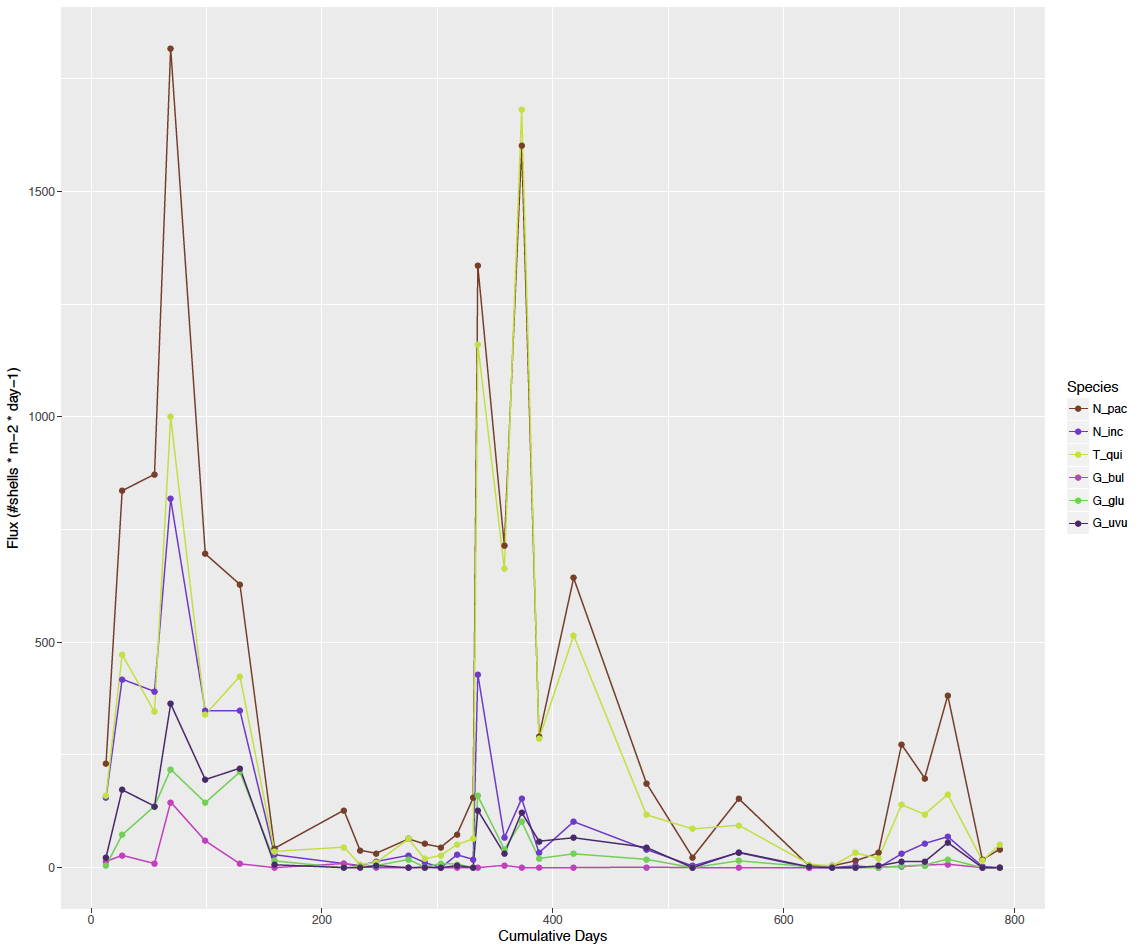
\includegraphics[width=1\textwidth]{NB67_series.png}
\caption{\label{fig:NB67_series} Example of data from trap no.1 (named NB67), colors represent species. This trap was active for 787 days, samples were taken in average every 18.2 days, with a total of 32 samples (Table \ref{table:traps_data})}
\end{figure}


\begin{figure}
\centering
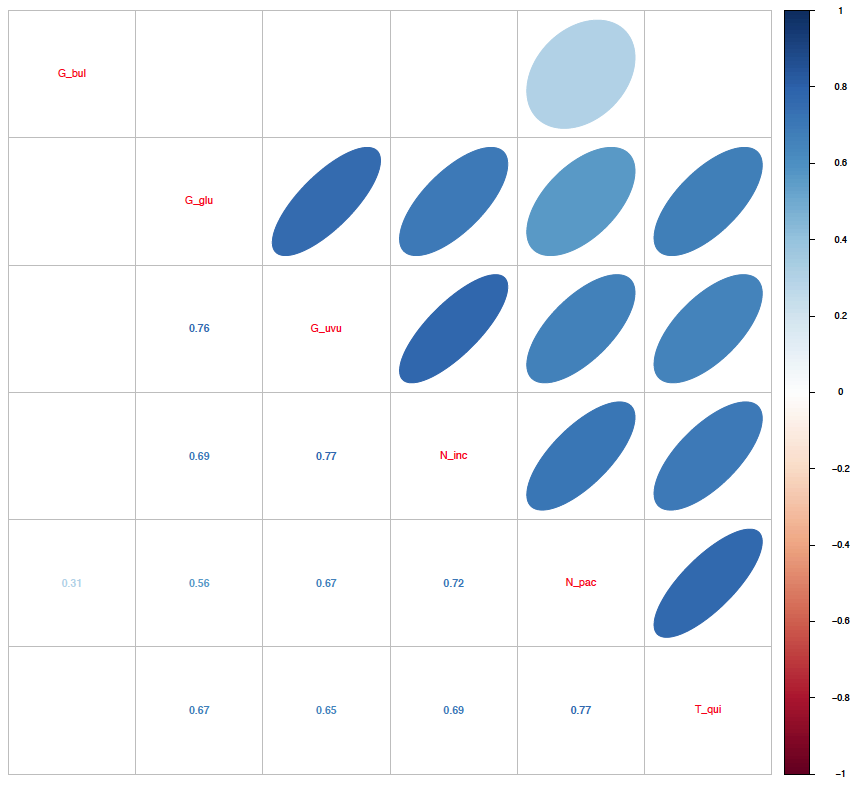
\includegraphics[width=0.7\textwidth]{NB67_corrplot_kendall_fd.png}
\caption{\label{fig:NB67_corrplot} Pair-wise Kendall correlation plot of first differences of time-series from Trap no.1 (NB67, Fig.\ref{fig:NB67_series}). Lower triangular matrix shows the correlation values and upper triangular matrix shows a representation of the correlation in form of elipses. R package corrplot \cite{wei2016corrplot}.}
\end{figure}



%----------------------------------------------------------------------------------------
\subsection{Null model (surrogates)}
The positive correlation among species might be an effect of seasonality. 
% another way to solve: function decompose in R,decompor a série temporal como uma soma de (trend + seasonality + noise) e subtrair a componente sazonal antes de fazer a análise. Porem, to do this, precisa botar a série no formato "time-series" do R. pra isso eh so usar a função "ts()", mas vc vai precisar saber o periodo (freq) da série.Pra achar o período, se não for nada óbvio (tipo anual) dá pra tentar chutar olhando as funções de autocorrelação e autocorrelação parcial (adf() e pacf() no R)
% "partial correlation": "the correlation between the residuals RX (X=ssp1) and RY (Y=ssp2) resulting from the linear regression with Z (Z = temperatura)"

For each time-series (\textit{i.e.}, each species in each sediment trap) we calculated a smoothing spline of the shell fluxes based on yearly observations. To do this, the observations were put on the same time-scale by converting the first date of the collection intervals to the day of the year. Then, a spline function was applied to the data.
We do not need to impose a priori the seasonality of the data with this methodology,and it allows for any number of shell flux peaks throughout the year.

The correlation between the time-series raw data and the spline series is an indicator of how seasonal the variable is. SST, for example, shows always a high correlation ($\rho$ ~ 0.9). We assume that if a species' shell flux responds to SST(or any other variable that relates to SST), its time-series will also be seasonal and show a high correlation with its splines. 

We generated a null model based on the splines of each time-series. For each time-step, we calculated the residual between the time-series data and the spline data, resulting in a vector of residuals with the same length as the time-series and the spline series. We then randomized the residuals 500 times (\textit{i.e.}, 500 different vectors) and added it to the base spline series. This resulted in 500 null series. We calculated the correlation between species pairs for this 500 null series, and the resulting correlation distribution was used as the null model which takes seasonality into account. 

If species correlate positively just because they have synchronous seasonality, then their splines should correlate positively as well. 



%----------------------------------------------------------------------------------------
\subsection{Empirical dynamic modelling and convergent cross mapping of the Gulf of Mexico sediment trap}

\subsubsection{Gulf of Mexico sediment trap}
The Gulf of Mexico (GoM, 27.5N -90.3E (= 269.7), \textcolor{red}{REF}) sediment trap has the best resolution of all the sediment traps compiled by \cite{jonkers2015global}. The resolution is one community sample every 7 days (\textit{i.e.} each sample represents the accumulation of foraminifera shells of the previous week). The total length of the GoM time-series is 238 samples, spanning over 2245 from 14th January 2008 to 8th March 2014.

\subsubsection{Temperature for the Gulf of Mexico sediment trap}
I used the dataset NOAA 1/4o daily Optimum Interpolation Sea Surface Temperature (or daily OISST, AVHRR-Only) \citep{smith2016oisst}.  % http://monitor.cicsnc.org/obs4MIPs/    https://www.ncdc.noaa.gov/oisst/data-access 
We used the temperature data point of coordinates (lon 269.625  lat 27.625) 15,76 km away from the sediment trap. 

I calculated the mean of the daily temperature for each sampling interval. The NOAA dataset has the temperature values in Kelvin, the Celsius column was created subtracting 273.15 from the Kelvin values. 
% Uma coisa a se pensar é que nossos dados da serie temporal são conchas de foraminiferos que morreram recentemente. Então, o indivíduo que morreu no dia X (ou antes do dia X, e só caiu na armadilha no dia X), não vivenciou a temperatura do dia X e sim dos dias anteriores. Como o tempo de vida médio de um indivíduo é um mês (obs.: isso não é completamente claro na literatura/campo), talvez seja melhor eu colocar os dados de temperatura de X-15 dias ou ate X - 30 dias. Eu poderia ja adicionar uma coluna extra tipo "temp_oC-15days". O que vocês acham?


\subsubsection{Empirical dynamic modelling and convergent cross mapping}
Empirical dynamic modelling (EDM) and convergent cross mapping (CCM), R package rEDM.




